%%%%%%%%%%%%%%%%%%%%%%%%%%%%%%%%%%%%%%%%%
% Masters/Doctoral Thesis 
% LaTeX Template
% Version 1.42 (19/1/14)
%
% This template has been downloaded from:
% http://www.latextemplates.com
%
% Original authors:
% Steven Gunn 
% http://users.ecs.soton.ac.uk/srg/softwaretools/document/templates/
% and
% Sunil Patel
% http://www.sunilpatel.co.uk/thesis-template/
%
% License:
% CC BY-NC-SA 3.0 (http://creativecommons.org/licenses/by-nc-sa/3.0/)
%
% Note:
% Make sure to edit document variables in the Thesis.cls file
%
%%%%%%%%%%%%%%%%%%%%%%%%%%%%%%%%%%%%%%%%%

%----------------------------------------------------------------------------------------
%	PACKAGES AND OTHER DOCUMENT CONFIGURATIONS
%----------------------------------------------------------------------------------------

\documentclass[12pt, a4paper, oneside]{Thesis} % Paper size, default font size and one-sided paper

\graphicspath{{Pictures/}} % Specifies the directory where pictures are stored

\usepackage[square, numbers, comma, sort&compress]{natbib} % Use the natbib reference package - read up on this to edit the reference style; if you want text (e.g. Smith et al., 2012) for the in-text references (instead of numbers), remove 'numbers' 

\usepackage{mdframed}
\usepackage{etoolbox}
\definecolor{secnum}{RGB}{13,151,225}
\hypersetup{urlcolor=blue, colorlinks=true} % Colors hyperlinks in blue - change to black if annoying

\definecolor{darkgreen}{rgb}{0,0.5,0}

\usepackage{algorithm}
\usepackage{algorithmic}
\usepackage{multirow}
\usepackage{graphicx}
\usepackage{listings} 
\usepackage{caption}


\title{\ttitle} % Defines the thesis title - don't touch this


\usepackage{titlesec}
% \usepackage{titletoc}
% \usepackage{xCJKnumb}
\titleformat{\chapter}{\Huge\bfseries}{Section\,{\thechapter}\hfill}{1em} {}

\begin{document}

\frontmatter % Use roman page numbering style (i, ii, iii, iv...) for the pre-content pages

\setstretch{2} % Line spacing of 1.3

% Define the page headers using the FancyHdr package and set up for one-sided printing
\fancyhead{} % Clears all page headers and footers
\rhead{\thepage} % Sets the right side header to show the page number
\lhead{} % Clears the left side page header

\pagestyle{fancy} % Finally, use the "fancy" page style to implement the FancyHdr headers

\newcommand{\HRule}{\rule{\linewidth}{0.5mm}} % New command to make the lines in the title page

% PDF meta-data
\hypersetup{pdftitle={\ttitle}}
\hypersetup{pdfsubject=\subjectname}
\hypersetup{pdfauthor=\authornames}
\hypersetup{pdfkeywords=\keywordnames}

%----------------------------------------------------------------------------------------
%	TITLE PAGE
%----------------------------------------------------------------------------------------


\begin{titlepage}
\begin{center}

\textsc{\LARGE \univname}\\[1.5cm] % University name
\textsc{\Large Final Year Project}\\[0.5cm] % Thesis type

\HRule \\[0.4cm] % Horizontal line
{\huge \bfseries \ttitle}\\[0.4cm] % Thesis title
\HRule \\[1.5cm] % Horizontal line
 
\begin{minipage}{0.4\textwidth}
\begin{flushleft} \large
\emph{Author:}\\
{\authornames} % Author name - remove the \href bracket to remove the link
\\{SID:52165928}
\end{flushleft}
\end{minipage}
\begin{minipage}[t]{0.4\textwidth}
\begin{flushright} \large
\emph{Supervisor:} \\
\href{http://www6.cityu.edu.hk/ma/people/profile/zhuangxs.htm}{\supname} % Supervisor name - remove the \href bracket to remove the link  
\end{flushright}
\end{minipage}\\[3cm]
 
\large \textit{A thesis submitted in fulfilment of the requirements\\ for the degree of \degreename}\\[0.3cm] % University requirement text
\textit{in the}\\[0.4cm]
\deptname\\[2cm] % Research group name and department name
 
{\large \today}\\[4cm] % Date
%\includegraphics{Logo} % University/department logo - uncomment to place it
 
\vfill
\end{center}

\end{titlepage}
%----------------------------------------------------------------------------------------
%	DECLARATION PAGE
%	Your institution may give you a different text to place here
%----------------------------------------------------------------------------------------

% \Declaration{

% \addtocontents{toc}{\vspace{1em}} % Add a gap in the Contents, for aesthetics

% I, \authornames, declare that this thesis titled, '\ttitle' and the work presented in it are my own. I confirm that:

% \begin{itemize} 
% \item[\tiny{$\blacksquare$}] This work was done wholly or mainly while in candidature for a research degree at this University.
% \item[\tiny{$\blacksquare$}] Where any part of this thesis has previously been submitted for a degree or any other qualification at this University or any other institution, this has been clearly stated.
% \item[\tiny{$\blacksquare$}] Where I have consulted the published work of others, this is always clearly attributed.
% \item[\tiny{$\blacksquare$}] Where I have quoted from the work of others, the source is always given. With the exception of such quotations, this thesis is entirely my own work.
% \item[\tiny{$\blacksquare$}] I have acknowledged all main sources of help.
% \item[\tiny{$\blacksquare$}] Where the thesis is based on work done by myself jointly with others, I have made clear exactly what was done by others and what I have contributed myself.\\
% \end{itemize}
 
% Signed:\\
% \rule[1em]{25em}{0.5pt} % This prints a line for the signature
 
% Date:\\
% \rule[1em]{25em}{0.5pt} % This prints a line to write the date
% }

% \clearpage % Start a new page

%----------------------------------------------------------------------------------------
%	QUOTATION PAGE
%----------------------------------------------------------------------------------------

% \pagestyle{empty} % No headers or footers for the following pages

% \null\vfill % Add some space to move the quote down the page a bit

% \textit{``Thanks to my solid academic training, today I can write hundreds of words on virtually any topic without possessing a shred of information, which is how I got a good job in journalism."}

% \begin{flushright}
% Dave Barry
% \end{flushright}

% \vfill\vfill\vfill\vfill\vfill\vfill\null % Add some space at the bottom to position the quote just right

% \clearpage % Start a new page

%----------------------------------------------------------------------------------------
%	ABSTRACT PAGE
%----------------------------------------------------------------------------------------

\addtotoc{Abstract} % Add the "Abstract" page entry to the Contents

\abstract{\addtocontents{toc}{\vspace{1em}} % Add a gap in the Contents, for aesthetics
In this paper, we study wavelet transform and its application in image denoising and image inpainting. In the denoising and inpainting experiments, two types of filter banks named orthogonal filter bank and tight framelet filter bank respectively are considered. Also, different values of the threshold function and decomposition levels are carefully selected as they are the key to optimal results attained in extensive simulations of image denoising and impainting. Section 2 demonstrates the main methods and algorithms used in the experiments and Section 3 concentrates on comparing the results of different filter banks. This paper focuses on the property of different filter banks and shows the advantages of redundancy property of tight framelet filter banks in image inpainting.

}

\clearpage % Start a new page


%----------------------------------------------------------------------------------------
%	ACKNOWLEDGEMENTS
%----------------------------------------------------------------------------------------

% \setstretch{1.3} % Reset the line-spacing to 1.3 for body text (if it has changed)

% \acknowledgements{\addtocontents{toc}{\vspace{1em}} % Add a gap in the Contents, for aesthetics

% The acknowledgements and the people to thank go here, don't forget to include your project advisor\ldots
% }
% \clearpage % Start a new page

%----------------------------------------------------------------------------------------
%	LIST OF CONTENTS/FIGURES/TABLES PAGES
%----------------------------------------------------------------------------------------

\pagestyle{fancy} % The page style headers have been "empty" all this time, now use the "fancy" headers as defined before to bring them back

\lhead{\emph{Contents}} % Set the left side page header to "Contents"
\tableofcontents % Write out the Table of Contents

\lhead{\emph{List of Figures}} % Set the left side page header to "List of Figures"
\listoffigures % Write out the List of Figures

% \lhead{\emph{List of Tables}} % Set the left side page header to "List of Tables"
% \listoftables % Write out the List of Tables

%----------------------------------------------------------------------------------------
%	ABBREVIATIONS
%----------------------------------------------------------------------------------------

% \clearpage % Start a new page

% \setstretch{1.5} % Set the line spacing to 1.5, this makes the following tables easier to read

% \lhead{\emph{Abbreviations}} % Set the left side page header to "Abbreviations"
% \listofsymbols{ll} % Include a list of Abbreviations (a table of two columns)
% {
% \textbf{LAH} & \textbf{L}ist \textbf{A}bbreviations \textbf{H}ere \\
% %\textbf{Acronym} & \textbf{W}hat (it) \textbf{S}tands \textbf{F}or \\
% }

%----------------------------------------------------------------------------------------
%	PHYSICAL CONSTANTS/OTHER DEFINITIONS
%----------------------------------------------------------------------------------------

% \clearpage % Start a new page

% \lhead{\emph{Physical Constants}} % Set the left side page header to "Physical Constants"

% \listofconstants{lrcl} % Include a list of Physical Constants (a four column table)
% {
% Speed of Light & $c$ & $=$ & $2.997\ 924\ 58\times10^{8}\ \mbox{ms}^{-\mbox{s}}$ (exact)\\
% % Constant Name & Symbol & = & Constant Value (with units) \\
% }

%----------------------------------------------------------------------------------------
%	SYMBOLS
%----------------------------------------------------------------------------------------

% \clearpage % Start a new page

% \lhead{\emph{Symbols}} % Set the left side page header to "Symbols"

% \listofnomenclature{lll} % Include a list of Symbols (a three column table)
% {
% $a$ & distance & m \\
% $P$ & power & W (Js$^{-1}$) \\
% % Symbol & Name & Unit \\

% & & \\ % Gap to separate the Roman symbols from the Greek

% $\omega$ & angular frequency & rads$^{-1}$ \\
% % Symbol & Name & Unit \\
% }

%----------------------------------------------------------------------------------------
%	DEDICATION
%----------------------------------------------------------------------------------------

% \setstretch{1.3} % Return the line spacing back to 1.3

% \pagestyle{empty} % Page style needs to be empty for this page

% \dedicatory{For/Dedicated to/To my\ldots} % Dedication text

% \addtocontents{toc}{\vspace{2em}} % Add a gap in the Contents, for aesthetics

%----------------------------------------------------------------------------------------
%	THESIS CONTENT - CHAPTERS
%----------------------------------------------------------------------------------------

\mainmatter % Begin numeric (1,2,3...) page numbering

\pagestyle{fancy} % Return the page headers back to the "fancy" style

% Include the chapters of the thesis as separate files from the Chapters folder
% Uncomment the lines as you write the chapters

% Chapter Template
\chapter{Introduction} % Main chapter title

\label{Chapter1} % Change X to a consecutive number; for referencing this chapter elsewhere, use \ref{ChapterX}

\lhead{Section 1. \emph{Introduction}} % Change X to a consecutive number; this is for the header on each page - perhaps a shortened title

%----------------------------------------------------------------------------------------
%	SECTION 1
%----------------------------------------------------------------------------------------

\section{Introduction to Wavelet Transform}

Generally speaking, a wave is defined to be an oscillating function of time or space, for example, sinusoid and cosinousoid are typical waves used in many fields such as Fourier analysis, which expands signals in terms of sinusiods. In reality, fourier transform has proven to be extremely useful in mathematics, science and engineering especially in dealing with periodic signals. A wavelet is a ``small wave'' with its energy concentrated at a small area and is examined to be more efficient in the analysis of nonstationary phenomena. Figure 1.1 and Figure 1.2 illustrate the main difference between a wave and a wavelet, where a wavelet has its finite energy concentrated around a point compared to wave.
% 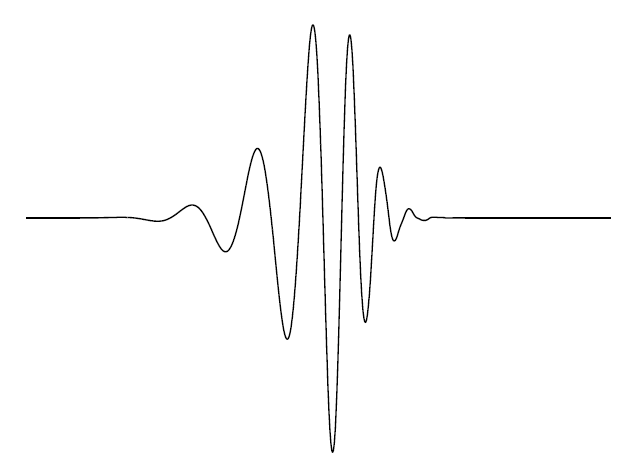
\includegraphics{wavelet.png}
 \begin{figure}[htb]
  \centering
  \begin{minipage}[c]{0.5\textwidth}
\centering
  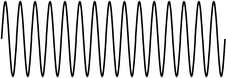
\includegraphics[width=1\linewidth]{sine-wave.png}
  \caption{A Sine Wave}
\end{minipage}%
%注意这个”%”绝对不能省,可以试试不打%的效果
\begin{minipage}[c]{0.5\textwidth}
\centering
  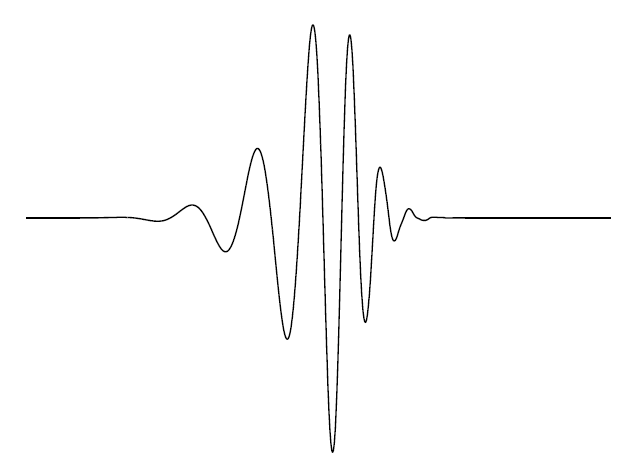
\includegraphics[width=0.6\linewidth]{wavelet.png}
  \caption{Daubechies' Wavelet $\psi_{D20}$}
  \end{minipage}

\end{figure}


%-----------------------------------
%	SUBSECTION 2
%-----------------------------------
\subsection{The Scaling Function}
Scaling functions are defined in order to implement the idea of multiresolution and wavelets are defined in terms of the scaling functions. Moreover, a two-dimensional family of scaling functions are transformed from basic scaling function through translation and scaling by
\begin{equation} \varphi_{j,k}(t) = 2^{j/2}\varphi(2^jt-k) \qquad  k \in \mathbb{Z} \qquad \varphi\in L^2  \end{equation}
and the subspace of $L^2(\mathbb{R})$ spanned by these functions is
\begin{equation} \mathcal{V}_j = \overline{Span_k\{\varphi_{j,k}(t) \}}  \end{equation}
In addition, scaling functions with a lower scale level can be expressed in terms of those at a higher scale by
\begin{equation} \varphi(t) = \sum_n h_0(n)\sqrt2\varphi(2t-n) \end{equation}

%-----------------------------------
%	SUBSECTION 2
%-----------------------------------

\subsection{The Wavelet Functions}
Instead of using $\varphi_{j,k}(t)$ and incresing $j$ to increase the size of the subspace spanned by those scaling functions, a slightly different set of functions $\psi_{j,k}(t)$ which span the differences between the spaces spanned by the various scales of the scaling function is defined by
\begin{equation} \psi(t) = \sum_n h_1(n)\sqrt{2}\varphi(2t-n) \qquad \end{equation}
A signal can be better described by the combination of scaling functions and wavelet functions, especially when the scaling functions and wavelets are orthogonal. Therefore, any function $f(t) \in L^2(\mathbb{R})$ can be represented as 
\begin{equation} f(t) = \sum_{k} c_{j_0}(k)\varphi_{j_0,k}(t) + \sum_k\sum_{j=j_0}^{\infty} d_j(k)\psi_{j,k}(t) \end{equation}


%----------------------------------------------------------------------------------------
%	SECTION 2
%----------------------------------------------------------------------------------------

\section{Introduction to Filter Banks and Discrete Wavelet Transform}
The coefficients $h_0(n)$ and $h_1(n)$ in the equations (1.3) and (1.4) can be viewed as digital filters and the coefficients $c_{j_0}(k)$ and $d_j(k)$ in equations (1.5) can be viewed as digital signals. In signal processing, filter banks contain analysis bank and synthesis bank. Orthogonal wavelet filter banks and tight framelet filter banks will be introduced in the next section and the efficiency of different filter banks will be studied through various experiments.
%-----------------------------------
%	SUBSECTION 2.1
%-----------------------------------

\subsection{Analysis - From Fine Scale to Coarse Scale}
In the process of Decomposition, analysis bank separates the input signal into multiple components with each one carrying different frequency sub-band of the original signal. These multiple components (a collection of sub-signals) can be used to emphasize aspects of the original signal and may help us work with the original signal in an easier and more efficient way. For instance, analysis banks are widely used in signal compression since most useless information can be easily discarded.
Given that $\varphi_{j,k}(t)$ and $\psi_{j,k}(t)$ are orthonormal, the $j^{th}$ level of scaling coefficients are derived from 
\begin{equation} c_j(k) = \langle f(t),\varphi_{j,k}(t)\rangle = \int f(t)2^{j/2}\varphi(2^jt-k)dt \end{equation}
Substituting $\varphi_{j,k}(t)$ with equation (1.1) giving the scaling coefficients
\begin{equation} c_j(k) = \sum_m h_0(m-2k)c_{j+1}(m) \end{equation}
The corresponding formula for the wavelet coefficients can be derived in the same way
\begin{equation} d_j(k) = \sum_m h_1(m-2k)c_{j+1}(m)\end{equation}

%-----------------------------------
%	SUBSECTION 2.2
%-----------------------------------
\subsection{Synthesis - From Coarse Scale to Fine Scale}
 The output of analysis can be reconstructed in the process of Reconstruction with the synthesis bank. Moreover, the desire for perfect reconstruction (i.e., the output signal is exactly the same as the input signal) imposes extra constraints on the analysis and synthesis filters.
 \begin{equation} c_{j+1}(k) = \sum_mc_j(m)h_0(k-2m) + \sum_md_j(m)h_1(k-2m) \end{equation}


%-----------------------------------
%	SUBSECTION 2.3
%-----------------------------------
 \subsection{Discrete Wavelet Transform}
 The classical discrete wavelet transform (DWT) provides means of implementing analysis on the basis of filter banks with the attribute of perfect reconstruction. It has proven to be practically efficient in the process of a certain classes of signals, especially for piecewise smooth signals which will be presented in the following sections. 




% Chapter Template

\chapter{Methods} % Main chapter title

\label{Chapter2} % Change X to a consecutive number; for referencing this chapter elsewhere, use \ref{ChapterX}

\lhead{Section 2. \emph{Methods}} % Change X to a consecutive number; this is for the header on each page - perhaps a shortened title

%----------------------------------------------------------------------------------------
%	SECTION 1
%----------------------------------------------------------------------------------------

\section{Discrete Framelet Transform}


%-----------------------------------
%	SUBSECTION 1
%-----------------------------------

\subsection{Mallat's algorithm}
The Mallat's algorithm was formally developed in 1988 by Mallat which proves to be a fast algorithm for wavelet decomposition and reconstruction. In the case of discrete wavelet transform, suppose that the length of the signal is $N = 2^J$, the transform can be efficiently computed by implementing Mallat's algorithm with the time complexity $O(N)$. Basically, the algorithm is a classical scheme for deriving the sub-signals using a set of low pass and high pass filters followed by a down-sampling process. To be specific, the low and high pass filters are predetermined by the mother wavelet. Moreover, the low pass filter generates the approximation coefficients and the output of the high pass filters is named detail coefficients. Figure 2.3 and Figure 2.5 shows the diagram of implementing the Mallat's algorithm. After the process of decomposition, the original signal is subsequently decomposed into several sub-signals with different scales.

%-----------------------------------
%	SUBSECTION 2
%-----------------------------------

\subsection{One Level Discrete Framelet Transform}

Equation (1.7) and equation (1.8) indicate that the scaling and wavelet coefficients at level of $j-1$ can be derived from convolving the expansion coefficients at scale $j$ by the coefficients $h_0(-n)$ and $h_1(-n)$ then down-sampling by two, which means taking even terms in the signal sequence and discard the odd terms. Namely, the scale-$j$ coefficients are filtered by two digital filters $h_0(n)$ and $h_1(n)$ and down-sampling the results gives the expansion coefficients at level of $j-1$.(as Figure 2.1 shows)

For the synthesis procedure, it is required to first up-sampling by two and then filtering, where up-sampling by two means inserting zeros between each of the original signal sequence.(as Figure 2.2 shows)
 \begin{figure}[h]
  \centering
  \begin{minipage}[c]{0.5\textwidth}
\centering
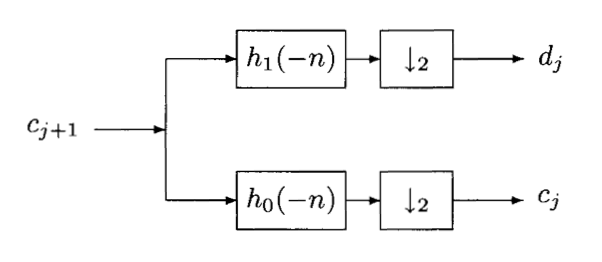
\includegraphics[width=.9\linewidth]{analysis_bank.png}
\caption{One Level Analysis Bank}
\end{minipage}%
%注意这个”%”绝对不能省,可以试试不打%的效果
\begin{minipage}[c]{0.5\textwidth}
\centering
  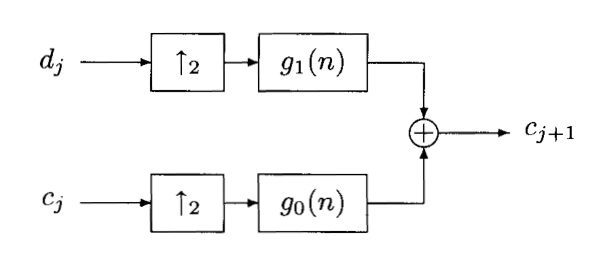
\includegraphics[width=0.9\linewidth]{synthesis_bank.png}
\caption{One Level Synthesis Bank}
  \end{minipage}

\end{figure}


As illustrated in section 1.2, one-level standard discrete framelet transform includes two separate steps named decomposition and reconstruction. Figure 2.3 shows the implementation of one-level discrete framelet transform with a dual framelet filter bank $\{u_0,...,u_s\},\{\tilde{u}_0,...,\tilde{u}_s\}$, the analysis filter $\{u_i\}$ plays the role of filtering the input signal while $\{\tilde{u}_i\}$ is the synthesis filter. The sub-signals are down-sampled after filtered so that the data rates will be the same in the sub-signals as in the original signal. To ease notation, the complex conjugate sequence of u reflected about the origin is denoted as $v^*$, which means $u^*(k) := \overline{u(-k)} $
\begin{figure}[htb]
\centering
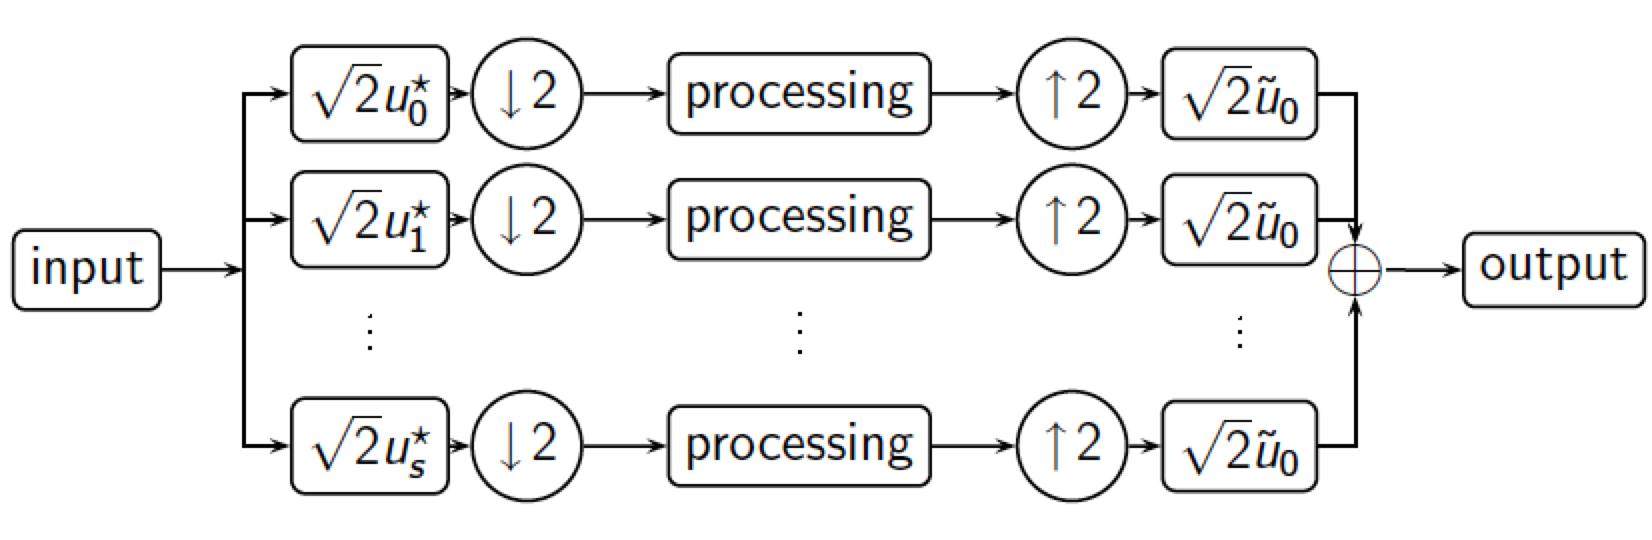
\includegraphics[width=.8\linewidth]{one_level.png}
\caption{Implementation of one-level discrete wavelet transform}
\end{figure}

%-----------------------------------
%	SUBSECTION 3
%-----------------------------------
\subsection{Multi-level discrete wavelet transform}

The filtering and down-sampling procedure can be repeated for several times on the scaling coefficients to give the multi-level structure as illustrated in Figure 2.4. Note that the total number of the sub-signal data will be the same as the number in original data as a result of the down-sampling process. Iterating the filter bank generates more subsets of sub-signals which can be reconstructed through the multi-level synthesis structure later on.
\begin{figure}[htb]
\centering
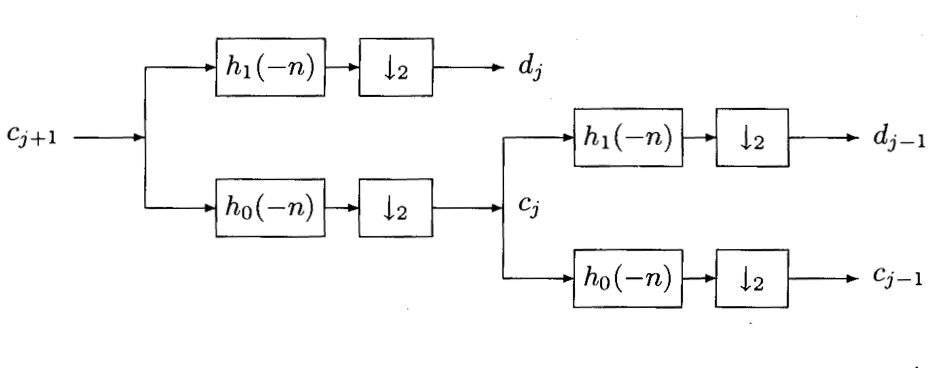
\includegraphics[width=.8\linewidth]{m_analysis_tree}
\caption{Two-level Analysis Tree}
\end{figure}

Figure 2.5 shows the implementation of a two-level discrete framelet transform with a dual framelet filter bank $ \{a,b_1,...,b_s\}, \{\tilde{a},\tilde{b}_1,...,\tilde{a}_s\}$ , also noting the value of the decomposition levels and of the reconstruction levels for a signal should be the same and is particularly determined by the user according to the characters of the original signal and the expected result.

\begin{figure}[htb]
\centering
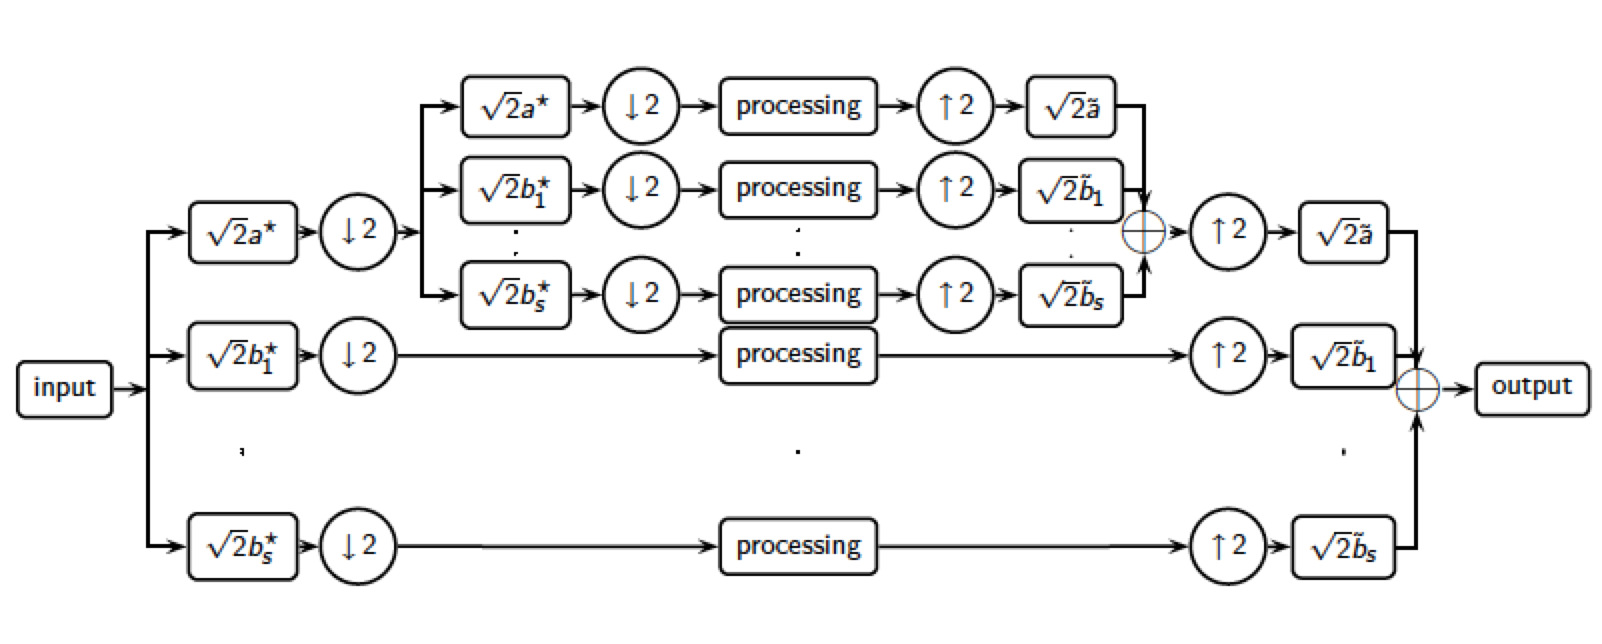
\includegraphics[width=.8\linewidth]{multi_level.png}
\caption{Two-level Discrete Framelet Transform}
\end{figure}


%-----------------------------------
%	SUBSECTION 4
%-----------------------------------

\subsection{Implement the algorithm on Images}
Images is interpreted as a two dimensional matrix with each element representing a pixel in the original image. Therefore, implementing discrete wavelet transform on images requires processing wavelet transform on rows and columns of the 2D matrix. Algorithm 1 briefly illustrates the method for implementing discrete framelet transform on images .


\begin{algorithm}  
\caption{Discrete Framelet Transform on Images}  
\label{alg:1}  
\begin{algorithmic}
\STATE $//$ Transform (Decomposition)
\STATE {parse image signal into a matrix C }
\FOR {each row in C}
\STATE {decompose the row signal according to levels of scale }   
\STATE sort the data into a row and store it into a new matrix D
\ENDFOR
\FOR {each column in C}
\STATE {decompose the column signal according to the same levels of scale}   
\STATE {sort the data into a column and store it into D}   
\ENDFOR
\STATE $//$ Inverse Transform (Reconstruction)
\FOR {each column in D}
\STATE using synthesis bank to reconstruct the column signal from the column in D
\ENDFOR
\FOR {each row in D}
\STATE using synthesis bank to reconstruct the row signal from the row in D
\ENDFOR

\end{algorithmic}  
\end{algorithm}  

Figure 2.6 shows the output of the decomposition process, the sub-bands are organized as rows and columns of the new matrix. With the low pass filter denoted as LP and the high pass filters denoted as HP, it is convenient to denote the output as shown in Figure 2.6. The sub-band $LL_3$ is called the low resolution residual and the others are named details.

\begin{figure}[htb]
\centering
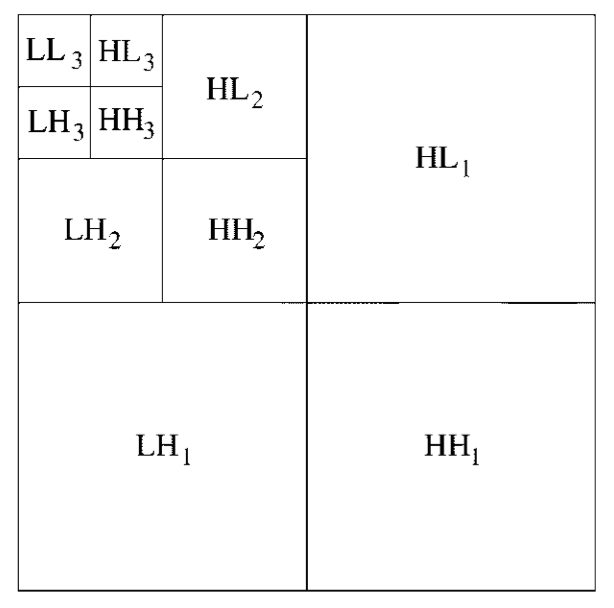
\includegraphics[width=.5\linewidth]{sub_bands.png}
\caption{Sub-bands of the 2D orthogonal wavelet transform}
\end{figure}

%----------------------------------------------------------------------------------------
%	SECTION 2
%----------------------------------------------------------------------------------------

\section{Wavelet Transform in Image Denoising}

It seems often that an image is corrupted by noise when it is transmitted. In that case, the main goal of image denoising is to discard the noise and retain the important signal features as much as possible. Recent work on image denoising through wavelet thresholding has indicated that various wavelet thresholding schemes and different thresholding values for denoising perform well and some of them have near-optimal properties.


\subsection{Problem Formulation}
Assume that there are $n$ noisy samples of function $f(t)$ in total, then denoising problem is usually posed as follows. 
\begin{equation} y_i = f(t_i) + \sigma\varepsilon_i, \qquad i=1,...,n  \end{equation}
Here $\varepsilon_i$ are independent and identically normal distributed $N(0,1)$ and $\sigma$ is called the noise level. As described, our goal is to discard the noise as much as possible and recover the function $f$, where the optimization criterion is the mean squared error (MSE). Namely, it is required to optimize $\hat{f}$ such that $\|\hat f - f\|_2 $ is minimized.

In the 2D scenario, peak signal-to-noise ratio, often abbreviated PSNR, is often used as the optimization criterion. PSNR is directly related to MSE and is defined to be
\begin{equation} PSNR = 10\cdot log_{10}(\frac{MAX^2_I}{MSE})  \end{equation}
where $MAX_I$ is the maximum possible pixel value of the image.

\subsection{Wavelet Thresholding}
Usually the output coefficients of the wavelet transform are sparse, in other words, most values in the coefficients are approximately zero in wavelet transform without the noise. Therefore, in the case of wavelet transform with noise, coefficients with small magnitude are typically noise and ought to be discarded in the denoising problem. The value used to identify noise in this approach is called threshold value and it determines whether a coefficient should be retained. The threshold value denoted by $\lambda$ is usually determined by the decomposition level $j$, e.g. $\lambda= \lambda(j)$

In practice, the thresholding method is only applied to the detail coefficients rather than the approximation coefficients since the approximation coefficients usually contain important components of the signal. Hard thresholding and soft thresholding are often used to thresholding the wavelet coefficients and the rules are given respectively as follows
\begin{eqnarray}
\delta^H_\lambda(d_{jk}) =
\begin{cases}
0       & |d_{jk}|\leqslant \lambda \\
d_{jk}   & |d_{jk}| > \lambda 
\end{cases}
\end{eqnarray}

\begin{eqnarray}
\delta^S_\lambda(d_{jk}) =
\begin{cases}
0       & |d_{jk}|\leqslant \lambda \\
d_{jk}-\lambda   & d_{jk} > \lambda \\
d_{jk}+\lambda   & d_{jk} < -\lambda 
\end{cases}
\end{eqnarray}


\subsection{Algorithm for image denoising}

\renewcommand{\algorithmicrequire}{ \textbf{Input:}} %Use Input in the format of Algorithm  
\renewcommand{\algorithmicensure}{ \textbf{Output:}} %UseOutput in the format of Algorithm  

\begin{algorithm}  
\caption{Image Denoising}  
\label{alg:2}  
\begin{algorithmic}
\REQUIRE ~~\\ %算法的输入参数:Input  
Original Image C; noise level $\sigma$; Decomposition level l; threshold value $\lambda$
\ENSURE ~~\\ %算法的输出:Output  
Image D Recovered from the noise; PSNR value;
\STATE {parse image signal into a matrix C }
\STATE add noise to the image C according to $\sigma$
\FOR {each row in C}
\STATE {decompose the row signal according to l }   
\STATE sort the data into a row and store it into a new matrix D
\ENDFOR
\FOR {each column in C}
\STATE {decompose the column signal according to l}   
\STATE {sort the data into a column and store it into D}   
\ENDFOR
\STATE hard/soft thresholding the matrix D according to $\lambda$
\STATE $//$ Inverse Transform (Reconstruction)
\FOR {each column in D}
\STATE using synthesis bank to reconstruct the column signal from the column in D
\ENDFOR
\FOR {each row in D}
\STATE using synthesis bank to reconstruct the row signal from the row in D
\ENDFOR
\STATE Calculate PSNR for C and D
\end{algorithmic}  
\end{algorithm}  

\begin{figure}[h]
\centering
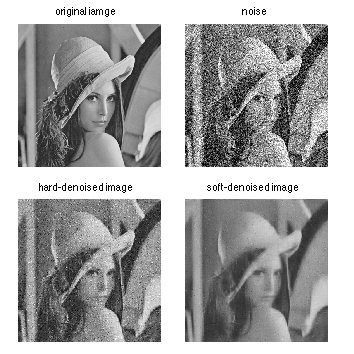
\includegraphics[width=.8\linewidth]{deno_eg.png}
\caption{Image Denoising using hard and soft thresholding with $\sigma = 50$}
\end{figure}



%----------------------------------------------------------------------------------------
%	SECTION 3
%----------------------------------------------------------------------------------------
\newpage
\section{Wavelet Transform in Image Inpainting}

\subsection{Problem Formulation}
Typically, inpainting is described as the way reconstructing deteriorated part of an image. An effective inpainting process involves application of sophisticated algorithms to replace the corrupted part of the image data. Compared to image denoising, a mask matrix representing the corrupted area of the image is required for image inpainting.

Given an image data matrix C and a region $\Omega$ inside it, the inpainting problem consists in reconstructing the data in $\Omega$ in order to eliminate some outstanding difference between the region and its surroundings. A complete process of image inpainting usually requires implementing the wavelet transform recursively for several times in order to reconstruct the image perfectly. Figure 2.8 shows the ouput of the implementation for image inpainting using both hard and soft thresholding.

\subsection{Algorithm for image inpainting}

\renewcommand{\algorithmicrequire}{ \textbf{Input:}} %Use Input in the format of Algorithm  
\renewcommand{\algorithmicensure}{ \textbf{Output:}} %UseOutput in the format of Algorithm  

\begin{algorithm}  
\caption{Image Inpainting}  
\label{alg:3}  
\begin{algorithmic}
\REQUIRE ~~\\ %算法的输入参数:Input  
Original Image C; Mask Matrix M;Recursion times n; Decomposition level l; threshold value $\lambda$
\ENSURE ~~\\ %算法的输出:Output  
Reconstructed Image; PSNR value;
\STATE {parse image signal into a matrix C }
\STATE read a mask M
\STATE C = A.*B is the image with missing information
\FOR {i = 1:n }
\FOR {each row in C}
\STATE {decompose the row signal according to l }   
\STATE sort the data into a row and store it into a new matrix D
\ENDFOR
\FOR {each column in C}
\STATE {decompose the column signal according to l}   
\STATE {sort the data into a column and store it into D}   
\ENDFOR
\STATE hard/soft thresholding the matrix D according to $\lambda$
\STATE $//$ Inverse Transform (Reconstruction)
\FOR {each column in D}
\STATE using synthesis bank to reconstruct the column signal from the column in D
\ENDFOR
\FOR {each row in D}
\STATE using synthesis bank to reconstruct the row signal from the row in D
\ENDFOR
\STATE Update the missing information of C by $C_{new}=(1-M).*D+M.*C$ and replace C by $C_{new}$
\STATE replace threshold value $\lambda$ by a smaller value
\ENDFOR
\STATE Calculate PSNR for C
\end{algorithmic}  
\end{algorithm}  

\begin{figure}[h]
\centering
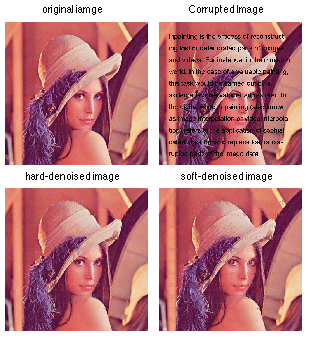
\includegraphics[width=.8\linewidth]{inp_eg.png}
\caption{Image Inpainting using hard and soft thresholding }
\end{figure}

 
% Chapter Template

\chapter{Results} % Main chapter title

\label{Chapter3} % Change X to a consecutive number; for referencing this chapter elsewhere, use \ref{ChapterX}

\lhead{Section 3. \emph{Results}} % Change X to a consecutive number; this is for the header on each page - perhaps a shortened title

%----------------------------------------------------------------------------------------
%	SECTION 1
%----------------------------------------------------------------------------------------

\section{Image Denoising}
\subsection{PSNR results in image denoising}

In order to assess the performance of various filter banks in image denoising, three images named Lena, Boat and Barbara respectively were chosen as the original image. Moreover, five different filter banks including two Daubechies filters and three tight framelet filters. In the following analysis, the ``Haar'' wavelet filter is referred as `db1' and the Daubechies 4-tap filter is referred as `db2'. Also, `tf1',`tf2' and `tf3' are representing three different kinds of tight framelet wavelet filters.
\begin{itemize}
    \item Orthogonal Filter Bank `db1' 
    \begin{itemize}
        \item $h_0 = \{\frac{1}{2},\frac{1}{2}\}$ \qquad $h_1 = \{-\frac{1}{2},\frac{1}{2}\}$
        \item $g_0 = \{\frac{1}{2},\frac{1}{2}\}$ \qquad $g_1 = \{-\frac{1}{2},\frac{1}{2}\}$

    \end{itemize}

    \item Orthogonal Filter Bank `db2' 
    \begin{itemize}
        \item $h_0 = \{\frac{1-\sqrt3}{8},\frac{-3+\sqrt3}{8},\frac{3+\sqrt3}{8},\frac{-1-\sqrt3}{8}\}$ \qquad $h_1 = \{\frac{1+\sqrt3}{8},\frac{3+\sqrt3}{8},\frac{3-\sqrt3}{8},\frac{1-\sqrt3}{8}\}$
        \item $g_0 = \{\frac{1-\sqrt3}{8},\frac{-3+\sqrt3}{8},\frac{3+\sqrt3}{8},\frac{-1-\sqrt3}{8}\}$ \qquad $g_1 = \{\frac{1+\sqrt3}{8},\frac{3+\sqrt3}{8},\frac{3-\sqrt3}{8},\frac{1-\sqrt3}{8}\}$
    \end{itemize}
    \item Tight Framelet Filter Bank `tf1' 
    \begin{itemize}
        \item $h_0 = \{\frac{1}{4},\frac{1}{2},\frac{1}{4}\}$ \qquad $h_1 = \{-\frac{\sqrt2}{4},0,\frac{\sqrt2}{4}\}$ \qquad $h_2 = \{-\frac{1}{4},\frac{1}{2},-\frac{1}{4}\}$
        \item $g_0 = \{\frac{1}{4},\frac{1}{2},\frac{1}{4}\}$ \qquad $g_1 = \{-\frac{\sqrt2}{4},0,\frac{\sqrt2}{4}\}$ \qquad $g_2 = \{-\frac{1}{4},\frac{1}{2},-\frac{1}{4}\}$
    \end{itemize}

    \item Tight Framelet Filter Bank `tf2' 
    \begin{itemize}

        \item $h_0 = \{\frac{5}{1024},0,-\frac{63}{1024},\frac{75}{1024},\frac{495}{1024},\frac{495}{1024},\frac{75}{1024},-\frac{63}{1024},0,\frac{5}{1024}\}$ \\ 
        $h_1 = \{0,0,-\frac{3\sqrt{15}}{512},0,\frac{22\sqrt{15}}{512},-\frac{45\sqrt{15}}{512},\frac{45\sqrt{15}}{512},-\frac{22\sqrt{15}}{512},0,\frac{3\sqrt{15}}{512}\}$ \\
        $h_2 = \{\frac{5}{1024},0,-\frac{117}{1024},\frac{75}{1024},\frac{315}{1024},-\frac{315}{1024},-\frac{75}{1024},\frac{117}{1024},0,-\frac{5}{1024}\}$ \\ 
        \item $g_0 = \{\frac{5}{1024},0,-\frac{63}{1024},\frac{75}{1024},\frac{495}{1024},\frac{495}{1024},\frac{75}{1024},-\frac{63}{1024},0,\frac{5}{1024}\}$ \\ 
        $g_1 = \{0,0,-\frac{3\sqrt{15}}{512},0,\frac{22\sqrt{15}}{512},-\frac{45\sqrt{15}}{512},\frac{45\sqrt{15}}{512},-\frac{22\sqrt{15}}{512},0,\frac{3\sqrt{15}}{512}\}$ \\
        $g_2 = \{\frac{5}{1024},0,-\frac{117}{1024},\frac{75}{1024},\frac{315}{1024},-\frac{315}{1024},-\frac{75}{1024},\frac{117}{1024},0,-\frac{5}{1024}\}$ \\ 
    \end{itemize}
    \item Tight Framelet Filter Bank `tf3' 
    \begin{itemize}
        \item $h_0 = \{\frac{63}{5120},0,-\frac{-429}{5120},0,\frac{1309}{5120},\frac{1617}{5120},\frac{1617}{5120},\frac{1309}{5120},0,-\frac{429}{5120},0,\frac{63}{5120}\}$ \\ 
        $h_1 = \{0,0,\frac{3\sqrt{231}}{2560},0,\frac{10\sqrt{231}}{2560},0,-\frac{77\sqrt{231}}{2560},\frac{77\sqrt{231}}{2560},0,-\frac{10\sqrt{231}}{2560},0,-\frac{3\sqrt{231}}{2560}\}$ \\
        $h_2 = \{\frac{63}{5120},0,-\frac{495}{5120},0,\frac{385}{5120},\frac{1617}{5120},-\frac{1617}{5120},-\frac{385}{5120},0,-\frac{495}{5120},0,-\frac{63}{5120}\}$ \\ 
        \item $g_0 = \{\frac{63}{5120},0,-\frac{-429}{5120},0,\frac{1309}{5120},\frac{1617}{5120},\frac{1617}{5120},\frac{1309}{5120},0,-\frac{429}{5120},0,\frac{63}{5120}\}$ \\ 
        $g_1 = \{0,0,\frac{3\sqrt{231}}{2560},0,\frac{10\sqrt{231}}{2560},0,-\frac{77\sqrt{231}}{2560},\frac{77\sqrt{231}}{2560},0,-\frac{10\sqrt{231}}{2560},0,-\frac{3\sqrt{231}}{2560}\}$ \\
        $g_2 = \{\frac{63}{5120},0,-\frac{495}{5120},0,\frac{385}{5120},\frac{1617}{5120},-\frac{1617}{5120},-\frac{385}{5120},0,-\frac{495}{5120},0,-\frac{63}{5120}\}$ \\ 

    \end{itemize}
\end{itemize}

In table 3.1, 3.2 and 3.3, the columns refer to five filter banks respectively and the rows represent cases in different noise levels. In the experiment, several possible combination of different coefficients (e.g. Decomposition Levels, Threshold values...) were tried in order to obtain the near optimal performance of a method as much as possible. Moreover, both soft thresholding and hard thresholding schemes were implemented and the results can be easily compared in the cells. Finally, the following three tables present the nearly optimal PSNR values for different methods and various noise levels. The result of the method with the best performance is highlighted in bold font for each test set.\\

\begin{algorithm} 
\caption{Obtaining the optimum denoising result}  
\label{alg:4}  
\begin{algorithmic}
\REQUIRE ~~\\ %算法的输入参数:Input  
A choices set L for possible levels (e.g. L= [3:7])
A choices set TV for possible threshold values (e.g. TV = [50:25:300])
\ENSURE ~~\\ %算法的输出:Output  
The optimum $PSNR_{opt}$ and the optimum Indices $i_{opt},j_{opt}$
\STATE let $PSNR_{opt} = 0$
\STATE let $i_{opt} , j_{opt} =0$
\FOR {i = 1: length(L)}
\STATE $l = L(i)$
\FOR {j = 1: length(TV)}
\STATE $th = TV(j)$
\STATE Using denoising algorithm to compute the PSNR with Decomposition levels = l and threshold value = th
\IF {$PSNR > PSNR_{opt}$}
\STATE $PSNR_{opt} = PSNR, \; i_{opt} = i,\; j_{opt} = j$ 
\ENDIF
\ENDFOR
\ENDFOR

\end{algorithmic}  
\end{algorithm}  
\vfill
% Please remember to add \use{multirow} to your document preamble in order to suppor multirow cells
\begin{table}[h]
\resizebox{1\textwidth}{!}{
\begin{tabular}{|c|l|l|l|l|l|l|l|l|l|l|}
\hline
\multirow{2}{*}{Lena} & \multicolumn{2}{|l}{db1} & \multicolumn{2}{|l}{db2} & \multicolumn{2}{|l}{tf1} & \multicolumn{2}{|l}{tf2} & \multicolumn{2}{|l|}{tf3} \\ \cline{2-11} 
 & hard & soft & hard & soft & hard & soft & hard & soft & hard & soft \\ \hline
 $\sigma=5$ & \bf{29.56} & 26.61 & 33.01 & 19.94 & 29.07 & 25.59 & 30.04 & 26.38 & 28.69 & 25.35 \\ \hline
 $\sigma=5$ & 29.43 & 26.61 & \bf{31.02} & 19.81 & 29.04 & 25.58 & 29.98 & 26.35 & 28.67 & 25.34 \\ \hline
 $\sigma=15$ & 28.91 & 26.65 & 28.76 & 19.63 &\bf{29.02} & 25.58 & 29.83 & 26.32 & 28.66 & 25.34 \\ \hline
 $\sigma=20$ & 27.04 & 26.65 & 26.06 & 19.36 & 28.92 & 25.56 & \bf{29.60} & 26.25 & 28.49 & 25.31 \\ \hline
 $\sigma=30$ & 26.00 & 25.98 & 21.67 & 18.69 & 27.80 & 25.51 & \bf{28.51} & 26.12 & 26.69 & 25.25 \\ \hline
 $\sigma=50$ & 23.85 & 23.45 & 17.51 & 16.68 & 25.54 & 24.60 & \bf{25.94} & 25.30 & 24.74 & 24.11 \\ \hline
 $\sigma=100$ & 18.43 & 19.98 & 11.60 & 12.47 & 21.78 & 20.59 & \bf{22.05} & 21.22 & 21.80 & 20.50 \\ \hline
 \end{tabular}}
\caption{Lena Denoising}
 \end{table}

% Boat
\begin{table}[h]
\resizebox{1\textwidth}{!}{
\begin{tabular}{|l|l|l|l|l|l|l|l|l|l|l|}
\hline
\multicolumn{1}{|c}{\multirow{2}{*}{Boat}} & \multicolumn{2}{|l}{db1} & \multicolumn{2}{|l}{db2} & \multicolumn{2}{|l}{tf1} & \multicolumn{2}{|l}{tf2} & \multicolumn{2}{|l|}{tf3} \\ \cline{2-11} 
\multicolumn{1}{|c|}{} & hard & soft & hard & soft & hard & soft & hard & soft & hard & soft \\ \hline
$\sigma=5$ & 28.28 & 25.49 & \bf{30.07} & 19.80 & 27.23 & 24.09 & 27.98 & 24.81 & 26.83 & 23.88 \\ \hline
$\sigma=10$ & 28.12 & 25.49 & \bf{28.88} & 19.70 & 27.23 & 24.09 & 27.91 & 24.79 & 26.83 & 23.87 \\ \hline
$\sigma=15$ & 27.68 & 25.52 & 27.33 & 19.54 & 27.20 & 24.08 & \bf{27.84} & 24.78 & 26.78 & 23.87 \\ \hline
$\sigma=20$ & 26.18 & 25.52 & 25.26 & 19.31 & 27.16 & 24.09 & \bf{27.67} & 24.76 & 26.69 & 23.87 \\ \hline
$\sigma=30$ & 24.81 & 25.02 & 22.09 & 18.67 & 26.29 & 24.03 & \bf{26.66} & 24.65 & 25.42 & 23.83 \\ \hline
$\sigma=50$ & 22.65 & 22.58 & 17.65 & 16.64 & 23.90 & 23.37 & \bf{24.28} & 23.86 & 23.29 & 22.97 \\ \hline
$\sigma=100$ & 17.99 & 19.57 & 11.71 & 12.34 & \bf{20.84} & 19.76 & 21.09 & 20.53 & \bf{20.84} & 19.63 \\ \hline
\end{tabular}}
\caption{Boat Denoising}
\end{table}


%Barbara
\begin{table}[h]
\resizebox{1\textwidth}{!}{
\begin{tabular}{|l|l|l|l|l|l|l|l|l|l|l|}
\hline
\multicolumn{1}{|c}{\multirow{2}{*}{Barbara}} & \multicolumn{2}{|l}{db1} & \multicolumn{2}{|l}{db2} & \multicolumn{2}{|l}{tf1} & \multicolumn{2}{|l}{tf2} & \multicolumn{2}{|l|}{tf3} \\ \cline{2-11} 
\multicolumn{1}{|c|}{} & hard & soft & hard & soft & hard & soft & hard & soft & hard & soft \\ \hline
$\sigma=5$ & 26.62 & 24.06 & \bf{29.65} & 19.50 & 25.32 & 22.96 & 26.65 & 23.67 & 25.48 & 22.98 \\ \hline
$\sigma=10$ & 26.48 & 24.10 & \bf{28.41} & 19.40 & 25.35 & 22.97 & 26.65 & 23.66 & 25.50 & 22.99 \\ \hline
$\sigma=15$ & 26.10 & 24.14 & \bf{26.82} & 19.25 & 25.41 & 22.98 & 26.58 & 23.66 & 25.50 & 23.00 \\ \hline
$\sigma=20$ & 24.92 & 24.17 & 24.84 & 19.04 & 25.41 & 23.00 & \bf{26.48} & 23.66 & 25.46 & 23.02 \\ \hline
$\sigma=30$ & 23.24 & 23.92 & 20.94 & 18.46 & 24.98 & 23.05 & \bf{25.81} & 23.65 & 24.52 & 23.05 \\ \hline
$\sigma=50$ & 21.72 & 21.76 & 17.14 & 16.61 & 22.87 & 22.72 & \bf{23.27} & 23.22 & 22.59 & 22.55 \\ \hline
$\sigma=100$ & 17.68 & 19.14 & 11.33 & 12.56 & 20.29 & 19.91 & \bf{20.58} & 20.18 & 20.39 & 19.89 \\ \hline
\end{tabular}}
\caption{Barbara Denoising}
\end{table}



%-----------------------------------
%	SUBSECTION 2
%-----------------------------------

\subsection{Performance analysis}
In terms of thresholding schemes, the choice of hard thresholding gives a better performance evaluated by PSNR. In contrast, soft thresholding generates a poorer result in almost every test case. As the optimum data highlighted in bold illustrates, the filter banks `db2' and `tf1' have demonstrated a great advantage in image denoising over the other filter banks. To be specific, the data indicates that the tight framelet filter banks are preferable in the circumstances with higher noise levels and `db2' is preferable in the cases with lower noise levels. Figure 3.1 shows the difference between methods using orthogonal filter bank `db2' and tight framelet filter bank `tf2' in the performance of denoising with $\sigma = 30$. Moreover, the second column gives the zoom in graphs in order to show the details.
\begin{figure}[H]
\begin{minipage}[t]{0.55\textwidth}
\centering
\resizebox{5cm}{5cm}{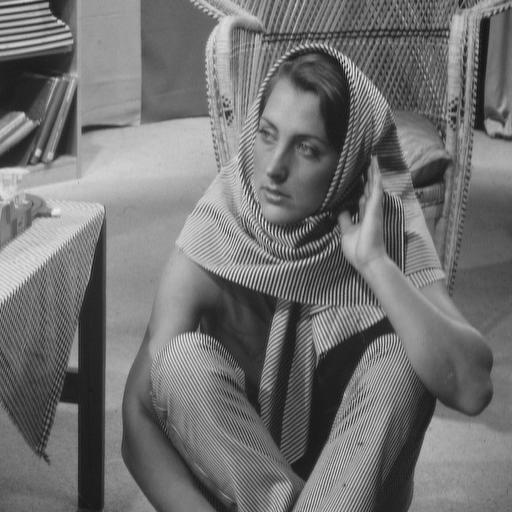
\includegraphics[width=.8\linewidth]{c1_1_1}}
\resizebox{5cm}{5cm}{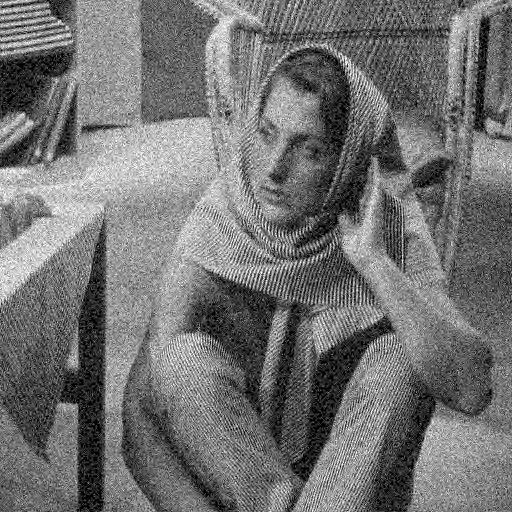
\includegraphics[width=.8\linewidth]{c1_2_1}}
\resizebox{5cm}{5cm}{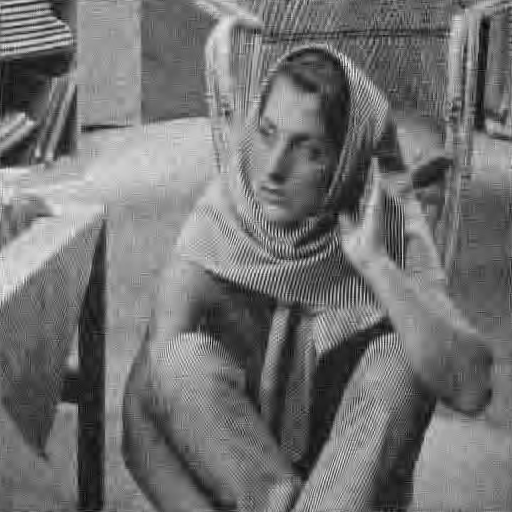
\includegraphics[width=.8\linewidth]{c1_3_1}}
\end{minipage}
\begin{minipage}[t]{0.5\textwidth}
\resizebox{5cm}{5cm}{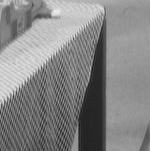
\includegraphics[width=1\linewidth]{c1_1_2}}
\resizebox{5cm}{5cm}{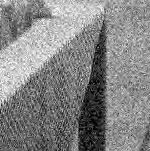
\includegraphics[width=1\linewidth]{c1_2_2}}
\resizebox{5cm}{5cm}{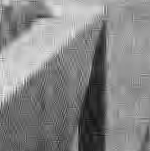
\includegraphics[width=1\linewidth]{c1_3_2}}
\end{minipage}
\caption{Denoising Result with $\sigma = 30$ for Barbara. Top: Original images and Zoom. Middle: `db2' Denoising. Bottom: `tf2' denoising.}
\end{figure}

%----------------------------------------------------------------------------------------
%	SECTION 2
%----------------------------------------------------------------------------------------

\section{Image Inpainting}
\subsection{PSNR results in image inpainting}
Inpainting process is more complicated than the denoising process in the way that recursive implementation is required for an effective inpainting process. Similar to the way we assessing the variables in denoising, several simple masks containing basic geometric graphs are selected and five filter banks are chosen in order to construct a comparision scheme. To further justify the choice of soft thresholding over hard thresholding in the process of inpainting, each test case is implemented for both thresholding methods. Similarly, the decomposition levels, initial threshold values and recursion times are selected form a range of feasible numbers for many times in order to reach the optimal result in extensive simulations.

\begin{figure}[H]
\begin{minipage}[t]{0.25\textwidth}
\resizebox{3.4cm}{3cm}{
\includegraphics[clip]{m_l_v}}\hspace{-0.4cm} 
\caption*{vertical line}
\resizebox{3.4cm}{3cm}{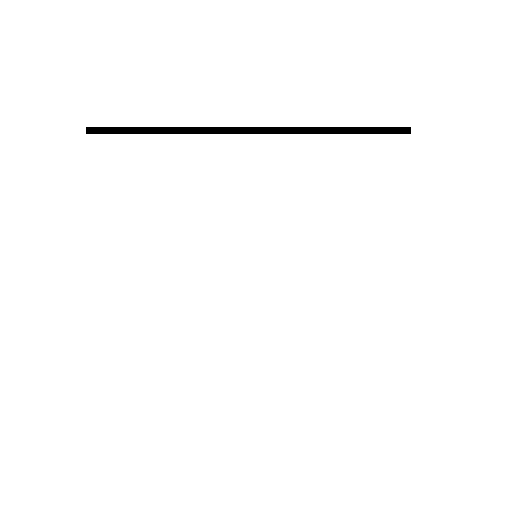
\includegraphics[clip]{m_l_h}}\hspace{-0.4cm} 
\caption*{horizontal line}
\end{minipage}\hspace{-0.2cm} 
\begin{minipage}[t]{0.25\textwidth}
\resizebox{3.4cm}{3cm}{
\includegraphics[clip]{m_l_rl}}\hspace{-0.4cm}
\caption*{right-left line}
\resizebox{3.4cm}{3cm}{
\includegraphics[clip]{m_l_lr}}\hspace{-0.4cm}
\caption*{left-right line}
\end{minipage}\hspace{-0.2cm} 
\begin{minipage}[t]{0.25\textwidth}
% \resizebox{6cm}{5cm}{\includegraphics{fig/p3/s_s2_1.eps}}\hfill
\resizebox{3.4cm}{3cm}{
\includegraphics[clip]{m_ring}}\hspace{-0.4cm}
\caption*{ring}
\resizebox{3.4cm}{3cm}{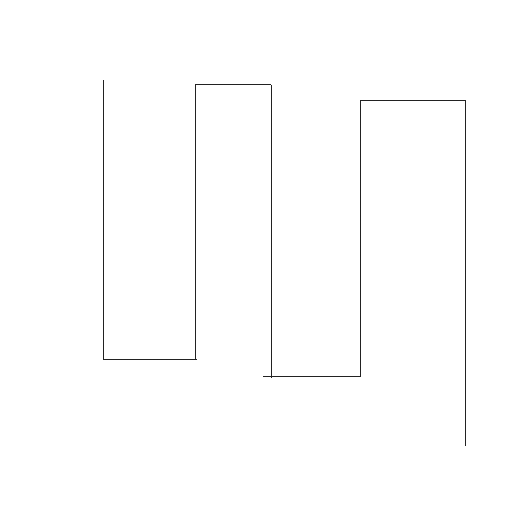
\includegraphics[clip]{m_line}}\hspace{-0.4cm}
\caption*{lines}
\end{minipage}\hspace{-0.2cm} 
\begin{minipage}[t]{0.25\textwidth}
\resizebox{3.4cm}{3cm}{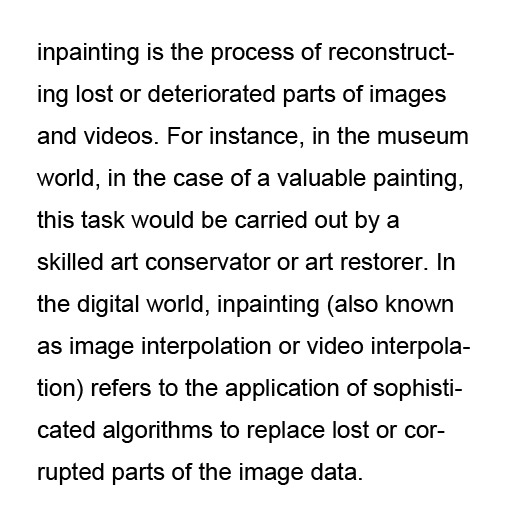
\includegraphics[clip]{m_text}}\hspace{-0.4cm}
\caption*{text}
\resizebox{3.4cm}{3cm}{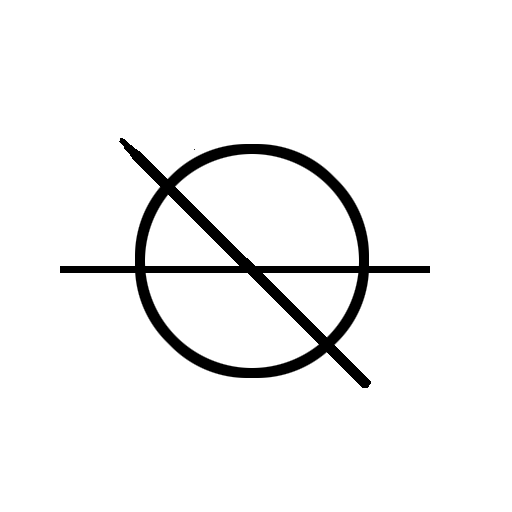
\includegraphics[clip]{m_combine}}
\caption*{combined mask}
\end{minipage}
\caption{Mask Figures}
\end{figure}

Figure 3.2 shows eight different masks used in our inpainting experiment including straight lines with four possible directions, a ring mask, text mask and a complicated mask combined of others. 


In the table 3.4, 3.5 and 3.6, the columns refer to fiver different filter banks, `db',`db2',`tf1',`tf2' and `tf3', the rows represent cases with different masks. And the second column named ``mask PSNR'' represent the corruption level of the mask image before the implementation of inpainting, surrounding values in the same row should be compared with the ``mask PSNR'' in order to justify the effectiveness of the corresponding method on the mask.\\

\begin{algorithm} 
\caption{Obtaining the optimum inpainting result}  
\label{alg:5}  
\begin{algorithmic}
\REQUIRE ~~\\ %算法的输入参数:Input  
A choices set L for possible levels (e.g. L= [3:7])
A choices set TV for possible threshold values (e.g. TV = [50:25:300])
A choices set R for possible recursion times (e.g. R =[3,5,7,9])
\ENSURE ~~\\ %算法的输出:Output  
The {opt}imum $PSNR_{opt}$ and the {opt}imum Indice $i_{opt},j_{opt}$
\STATE let $PSNR_{opt} = 0$
\STATE let $i_{opt} , j_{opt} =0, k_{opt} =0$
\FOR {i = 1: length(L)}
\STATE $l = L(i)$
\FOR {j = 1: length(TV)}
\STATE $th = TV(j)$
\FOR {k = 1: length(R)}
\STATE $rt = R(k)$
\STATE Using inpainting algorithm to compute the PSNR with Decomposition levels = l, threshold value = th, recursion time = rt
\IF {$PSNR > PSNR_{opt}$}
\STATE $PSNR_{opt} = PSNR, \; i_{opt} = i,\; j_{opt} = j, k_{opt} = k$ 
\ENDIF
\ENDFOR
\ENDFOR
\ENDFOR

\end{algorithmic}  
\end{algorithm}  

%Lena
% Please remember to add \use{multirow} to your document preamble in order to suppor multirow cells
\begin{table}[h]
\resizebox{1\textwidth}{!}{
\begin{tabular}{|l|l|l|l|l|l|l|l|l|l|l|l|}
\hline
\multicolumn{1}{|c}{\multirow{2}{*}{Lena}} & \multicolumn{1}{|c|}{\multirow{2}{*}{\begin{tabular}[c]{@{}c@{}}mask\\ PSNR\end{tabular}}} & \multicolumn{2}{|l}{db1}  & \multicolumn{2}{|l}{db2} & \multicolumn{2}{|l}{tf1} & \multicolumn{2}{|l}{tf2} & \multicolumn{2}{|l|}{tf3} \\ \cline{3-12} 
\multicolumn{1}{|c|}{} &  & hard & soft & hard & soft & hard & soft & hard & soft & hard & soft \\ \hline
vertical line   & 26.88 & 27.21 & 33.70 & 26.77 & 26.75 & 28.96 & 36.58 & 29.31 & 36.05 & 29.37 & \bf{36.62} \\ \hline
horizontal line & 24.39 & 24.65 & 32.43 & 25.03 & 24.98 & 25.81 & 37.00 & 25.91 & 39.16 & 26.51 & \bf{40.66} \\ \hline
right-left line & 23.01 & 25.75 & 32.03 & 23.32 & 23.29 & \bf{34.13} & 33.72 & 28.89 & 33.94 & 33.35 & 33.58 \\ \hline
left-right line & 24.62 & 27.92 & 32.99 & 24.98 & 24.87 & 38.41 & 37.82 & 33.03 & 37.37 & \bf{39.51} & 38.41 \\ \hline
ring            & 21.44 & 23.57 & 28.78 & 21.64 & 21.64 & 29.87 & 33.52 & 25.69 & 31.39 & 29.21 & \bf{33.72} \\ \hline
lines           & 27.18 & 28.51 & 43.32 & 33.69 & 32.64 & 32.74 & 43.36 & 37.23 & \bf{44.86} & 34.79 & 43.67 \\ \hline
text            & 15.75 & 26.52 & 30.95 & 16.08 & 16.13 & 33.75 & 33.13 & 33.71 & \bf{34.02} & 33.87 & 33.55 \\ \hline
combine         & 19.23 & 21.36 & 26.65 & 19.43 & 19.42 & 27.22 & \bf{31.39} & 24.16 & 30.50 & 27.00 & 31.25 \\ \hline
\end{tabular}}
\caption{Lena Inpainting}
\end{table}

%Boat
\begin{table}[h]
\resizebox{1\textwidth}{!}{
\begin{tabular}{|l|l|l|l|l|l|l|l|l|l|l|l|}
\hline
\multicolumn{1}{|c}{\multirow{2}{*}{Boat}} & \multicolumn{1}{|c|}{\multirow{2}{*}{\begin{tabular}[c]{@{}c@{}}mask\\ PSNR\end{tabular}}} & \multicolumn{2}{|l}{db1} & \multicolumn{2}{|l}{db2} & \multicolumn{2}{|l}{tf1} & \multicolumn{2}{|l}{tf2} & \multicolumn{2}{|l|}{tf3} \\ \cline{3-12} 
\multicolumn{1}{|c|}{} &  & hard & soft & hard & soft & hard & soft & hard & soft & hard & soft \\ \hline
vertical line   & 25.76 & 26.16 & 34.27 & 25.76 & 25.64 & 28.50 & 40.99 & 28.10 & 41.23 & 29.28 & \bf{41.28} \\ \hline
horizontal line & 24.96 & 25.22 & 33.91 & 25.60 & 25.55 & 26.44 & 39.68 & 26.35 & \bf{41.08} & 27.24 & 41.04 \\ \hline
right-left line & 23.39 & 26.26 & 31.67 & 23.66 & 23.63 & \bf{34.96} & 34.39 & 29.86 & 33.39 & 34.74 & 34.09 \\ \hline
left-right line & 23.39 & 26.29 & 33.45 & 23.73 & 23.67 & \bf{38.43} & 37.86 & 30.15 & 36.98 & 36.84 & 38.18 \\ \hline
ring            & 22.30 & 24.51 & 29.43 & 22.55 & 22.54 & 31.43 & 33.86 & 27.09 & 32.54 & 30.49 & \bf{34.16} \\ \hline
lines           & 27.28 & 28.73 & 42.03 & 32.67 & 32.15 & 33.87 & 41.59 & 37.06 & 43.01 & 35.75 & \bf{41.73} \\ \hline
text            & 15.39 & 26.73 & 30.39 & 15.72 & 15.73 & \bf{32.53} & 32.08 & 32.00 & 32.51 & 31.68 & 31.92 \\ \hline
combine         & 18.96 & 20.81 & 24.85 & 19.14 & 19.13 & 24.80 & \bf{29.38} & 22.79 & 28.50 & 24.90 & 29.26 \\ \hline
\end{tabular}}
\caption{Boat Inpainting}
\end{table}

%Barbara

\begin{table}[h]
\resizebox{1\textwidth}{!}{
\begin{tabular}{|l|l|l|l|l|l|l|l|l|l|l|l|}
\hline
\multicolumn{1}{|c}{\multirow{2}{*}{Barbara}} & \multicolumn{1}{|c|}{\multirow{2}{*}{\begin{tabular}[c]{@{}c@{}}mask\\ PSNR\end{tabular}}} & \multicolumn{2}{|l}{db1} & \multicolumn{2}{|l}{db2} & \multicolumn{2}{|l}{tf1} & \multicolumn{2}{|l}{tf2} & \multicolumn{2}{|l|}{tf3} \\ \cline{3-12} 
\multicolumn{1}{|c|}{} &  & hard & soft & hard & soft & hard & soft & hard & soft & hard & soft \\ \hline
vertical line   & 25.14 & 25.34 & 32.71 & 25.12 & 25.02 & 26.80 & \bf{45.54} & 26.44 & 42.06 & 27.06 & 43.35 \\ \hline
horizontal line & 25.49 & 25.79 & 31.95 & 26.13 & 26.07 & 26.76 & 36.31 & 27.31 & 36.39 & 27.53 & \bf{37.81} \\ \hline
right-left line & 24.37 & 27.62 & 33.38 & 24.63 & 24.60 & \bf{37.67} & 37.30 & 32.55 & 36.54 & 37.44 & 37.06 \\ \hline
left-right line & 22.92 & 25.66 & 32.37 & 23.22 & 23.17 & 36.19 & 35.97 & 29.52 & 35.79 & \bf{36.10} & 35.92 \\ \hline
ring            & 20.85 & 23.05 & 28.11 & 21.09 & 21.08 & 29.79 & 33.39 & 25.34 & 32.07 & 28.84 & \bf{33.70} \\ \hline
lines           & 27.53 & 29.18 & 40.95 & 31.12 & 31.92 & 34.52 & 40.84 & 39.67 & \bf{43.05} & 36.72 & 41.32 \\ \hline
text            & 16.31 & 26.98 & 30.03 & 16.54 & 16.59 & \bf{32.30} & 31.72 & 31.69 & 32.17 & 32.49 & 32.01 \\ \hline
combine         & 18.02 & 19.91 & 24.72 & 18.21 & 18.19 & 24.78 & 30.36 & 22.43 & 28.71 & 24.72 & 30.19 \\ \hline
\end{tabular}}
\caption{Barbara Inpainting}
\end{table}


\subsection{Performance analysis}
In terms of thresholding schemes,  the soft thresholding method shows a slight advantage in the process of image inpainting, whereas the hard thresholding also gets credit in some circumstances. As the optimal data highlighted in bold illustrates, the family of tight framelet filter banks demonstrated a great advantage in each test case. Figure 3.3 shows the comparison of inpainting results with text mask using orthogonal filter bank Haar and the tight framelet filter bank `tf1' correspondingly, and the second column shows the zoom in details. As we see, tight framelet filter bank is an effective tool since it has the property of redundancy and Figure 3.3 also indicates redundancy is desirable in some applications such as image inpainting. 
\begin{figure}[H]
\begin{minipage}[t]{0.5\textwidth}
\centering
\resizebox{5cm}{5cm}{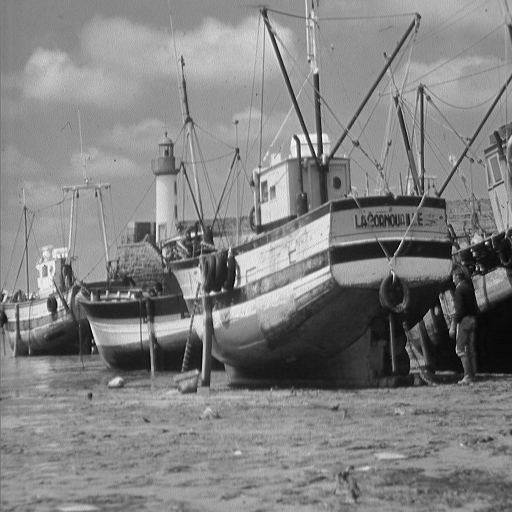
\includegraphics[width=.8\linewidth]{c2_1_1}}
\resizebox{5cm}{5cm}{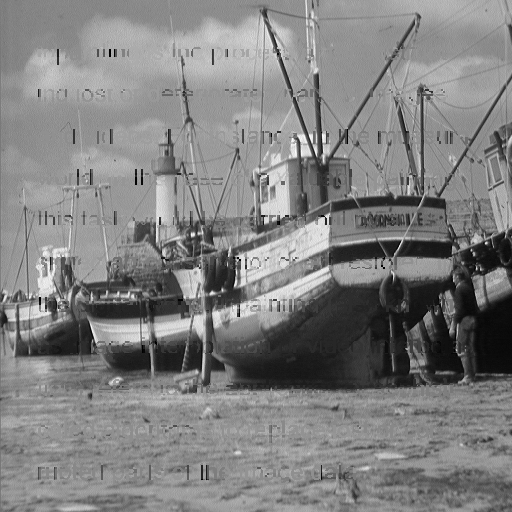
\includegraphics[width=.8\linewidth]{c2_2_1}}
\resizebox{5cm}{5cm}{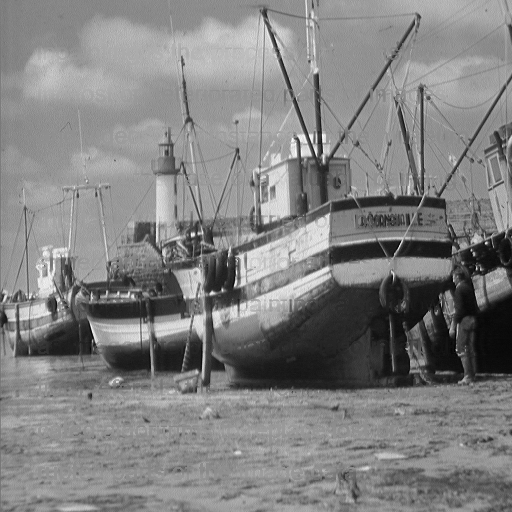
\includegraphics[width=.8\linewidth]{c2_3_1}}
\end{minipage}
\begin{minipage}[t]{0.5\textwidth}
\resizebox{5cm}{5cm}{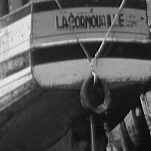
\includegraphics[width=1\linewidth]{c2_1_2}}
\resizebox{5cm}{5cm}{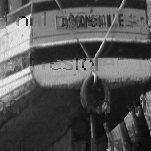
\includegraphics[width=1\linewidth]{c2_2_2}}
\resizebox{5cm}{5cm}{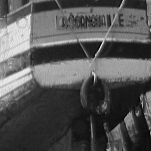
\includegraphics[width=1\linewidth]{c2_3_2}}
\end{minipage}
\caption{Inpainting Result with `text' mask for Boat. Top: Original images and Zoom. Middle: `db1' Inpainting. Bottom: `tf1' inpainting.}
\end{figure}

% Chapter Template

\chapter{Conclusion} % Main chapter title

\label{SectionX} % Change X to a consecutive number; for referencing this chapter elsewhere, use \ref{SectionX}

\lhead{Section 4. \emph{Conclusion}} % Change X to a consecutive number; this is for the header on each page - perhaps a shortened title

%----------------------------------------------------------------------------------------
%	SECTION 1
%----------------------------------------------------------------------------------------

In the applications of wavelet transform such as image denoising and image inpainting, careful choice of a suitable filter bank as well as coefficients such as threshold values and decomposition values can be very essential for obtaining a desirable result. Theoretically, frames are an over-complete version of a basis set and the tight frames are regarded as an over-complete version of an orthogonal basis set. 

In practical, the algorithms and computing methods used for different filter banks are basically the same, while the implementation with the tight framelet method can result in a certain amount of redundancy. However, this redundancy property of a tight framelet is desirable in the application of image inpainting since it gives a robustness in the transform and the errors consequently become less destructive. In the context of image denoising, the redundancy property seems not so effective as it behaves in the inpainting. Moreover, tight framelet filter banks are proved to be undesirable in denoising especially when the noise level is low (As shown in table 3.1).

\vfill
 
% % Chapter 1

\chapter{Chapter Title Here} % Main chapter title

\label{Chapterx} % For referencing the chapter elsewhere, use \ref{Chapter1} 

\lhead{Chapter 1. \emph{Chapter Title Here}} % This is for the header on each page - perhaps a shortened title

%----------------------------------------------------------------------------------------



%----------------------------------------------------------------------------------------

%----------------------------------------------------------------------------------------

\section{Thesis Features and Conventions}\label{ThesisConventions}


\subsection{References}

The `\texttt{natbib}' package is used to format the bibliography and inserts references such as this one \citep{Reference3}. The options used in the `\texttt{Thesis.tex}' file mean that the references are listed in numerical order as they appear in the text. Multiple references are rearranged in numerical order (e.g. \citep{Reference2, Reference1}) and multiple, sequential references become reformatted to a reference range (e.g. \citep{Reference2, Reference1, Reference3}).  
%\input{Chapters/Chapter5} 
%\input{Chapters/Chapter6} 
%\input{Chapters/Chapter7} 


%----------------------------------------------------------------------------------------
%	BIBLIOGRAPHY
%----------------------------------------------------------------------------------------

\label{Bibliography}

\lhead{\emph{Bibliography}} % Change the page header to say "Bibliography"

% \bibliographystyle{unsrtnat} % Use the "unsrtnat" BibTeX style for formatting the Bibliography

% \bibliography{Bibliography} % The references (bibliography) information are stored in the file named "Bibliography.bib"

\begin{thebibliography}{99} 
\bibitem {} B. Han and X. Zhuang, Algorithms for matrix extension and orthogonal wavelet filter banks over algebraic number fields, Mathematics of Computation. 82(281): 459-490, 2013
\bibitem {} B. Han and X. Zhuang, Matrix extension with symmetry and its applications to symmetric orthonormal multiwavelets. SIAM Journal on Mathematical Analysis. 42(5): 2297-2317, 2010
\bibitem {} B. Han, Properties of discrete framelet transforms, Mathematical Modelling of Natural Phenomena, 8, 18-47, 2013
\bibitem {} C. Sidney Burrus, Ramesh A. Gopinath and Haitao Guo, Introduction to Wavelets and Wavelet Transforms, Prentice Hall, 1998.
\bibitem {} C. K. Chui, An introduction to wavelets. Academic Press, Inc., Boston, MA, 1992.
\bibitem {} D. L. Donoho, Denoising by soft-thresholding, IEEE Transactions on Information Theory. Theory, 41, pp. 613–627, May 1995.
\bibitem {} F. Abramovich, T. Sapatinas, and B. W. Silverman, Wavelet thresh- olding via a Bayesian approach  J. R. Statist. Soc., 60, pp. 725–749, 1998.
\bibitem {} G. Strang and T. Nguyen, Wavelets and filter banks, Wellesley College, 2nd edition, 1996.
\bibitem {} I. Daubechies. Different Perspectives on Wavelets. American Mathematical Society, 47, January 11-12,1993.
\bibitem {} I. Daubechies. Ten lectures on wavelets. CBMS-NSF Regional Conference Series in Applied Mathematics, 61, December 1992.
\bibitem {} J. S. Walker and Ying-Jui Chen. Image denoising using tree-based wavelet subband correlations and shrinkage. Opt. Eng. 39, 2000.

\bibitem {} M. Steinbuch and M.J.G. van de Molengraft. Wavelet theory and applications: A literature study. Technical report, Eindhoven University of Technology, 2005. 
\bibitem {} Q. Mo and X. Zhuang, Matrix splitting with symmetry and dyadic framelet filter banks over algebraic number fields,  Linear Algebra and Its Applications, 437(10): 2650-2679, May 2012. 
\bibitem {} S. Mallat, A wavelet tour of signal processing. Third edition. Elsevier/Academic Press, Amsterdam, 2009.
\bibitem {} S. Tsai. Wavelet transform and denoising. Master’s thesis, Chapter 4, pp. 35-42, 2002.
\bibitem {} S. Grace Chang, Bin Yu, and Martin Vetterli, Adaptive Wavelet Thresholding for Image Denoising and Compression, IEEE Transactions On Image Processing, 9(9), September 2000.

\end{thebibliography}

%----------------------------------------------------------------------------------------
%	THESIS CONTENT - APPENDICES
%----------------------------------------------------------------------------------------

\addtocontents{toc}{\vspace{2em}} % Add a gap in the Contents, for aesthetics

\appendix % Cue to tell LaTeX that the following 'chapters' are Appendices

% Include the appendices of the thesis as separate files from the Appendices folder
% Uncomment the lines as you write the Appendices

% Appendix A
\titleformat{\chapter}{\centering\Huge\bfseries}{Appendix \,{\thechapter}}{1em} {}

\chapter{Some Important Matlab codes} % Main appendix title

\label{AppendixA} % For referencing this appendix elsewhere, use \ref{AppendixA}

\lhead{Appendix A. \emph{Some Important Matlab Codes}} % This is for the header on each page - perhaps a shortened title


\lstset{language=Matlab,
        basicstyle=\ttfamily\scriptsize,
        keywordstyle=\color{blue}\ttfamily,
        stringstyle=\color{red}\ttfamily,
        commentstyle=\color{darkgreen}\ttfamily,
        breaklines=true
}

\setstretch{1.2} % Line spacing of 1.3

\textbf{Funtion} \textit{Subdivision.m} 
\lstinputlisting{/Users/andywang/Documents/MATLAB/Subdivision.m}
\textbf{Funtion} \textit{Transition.m} 
\lstinputlisting{/Users/andywang/Documents/MATLAB/Transition.m}
\textbf{Funtion} \textit{Decomposition.m} 
\lstinputlisting{/Users/andywang/Documents/MATLAB/Decomposition.m}
\textbf{Funtion} \textit{Reconstruction.m} 
\lstinputlisting{/Users/andywang/Documents/MATLAB/Reconstruction.m}
\textbf{Funtion} \textit{multiLevel\_DFrT.m} 
\lstinputlisting{/Users/andywang/Documents/MATLAB/multiLevel_DFrT.m}
\textbf{Funtion} \textit{D2\_dwt.m} 
\lstinputlisting{/Users/andywang/Documents/MATLAB/D2_dwt.m}
\textbf{Funtion} \textit{D2\_idwt.m} 
\lstinputlisting{/Users/andywang/Documents/MATLAB/D2_idwt.m}
\textbf{Funtion} \textit{decreaseTV.m} 
\lstinputlisting{/Users/andywang/Documents/MATLAB/decreaseTV.m}
\textbf{Funtion} \textit{matchFilter.m} 
\lstinputlisting{/Users/andywang/Documents/MATLAB/matchFilter.m}
\textbf{Funtion} \textit{psnr.m} 
\lstinputlisting{/Users/andywang/Documents/MATLAB/psnr.m}
\textbf{Funtion} \textit{fconv.m} 
\lstinputlisting{/Users/andywang/Documents/MATLAB/fconv.m}
\textbf{Funtion} \textit{test\_deno.m} 
\lstinputlisting{/Users/andywang/Documents/MATLAB/test_deno.m}
\textbf{Funtion} \textit{test\_inp.m} 
\lstinputlisting{/Users/andywang/Documents/MATLAB/test_inp.m}
\textbf{Funtion} \textit{test\_inp\_c.m} 
\lstinputlisting{/Users/andywang/Documents/MATLAB/test_inp_c.m}
\textbf{Funtion} \textit{auto\_test\_deno.m} 
\lstinputlisting{/Users/andywang/Documents/MATLAB/auto_test_deno.m}
\textbf{Funtion} \textit{auto\_test\_inp.m} 
\lstinputlisting{/Users/andywang/Documents/MATLAB/auto_test_inp.m}

% \input{Appendices/AppendixB}
%\input{Appendices/AppendixC}

\addtocontents{toc}{\vspace{2em}} % Add a gap in the Contents, for aesthetics

\backmatter
\end{document}  